% Template for ISBI-2013 paper; to be used with:
%          spconf.sty  - ICASSP/ICIP LaTeX style file, and
%          IEEEbib.bst - IEEE bibliography style file.
% --------------------------------------------------------------------------
\documentclass{article}
\usepackage{spconf,amsmath,graphicx}
\usepackage{epstopdf}
\usepackage{epsfig}
\usepackage{amsfonts}
\usepackage{amssymb}
\newcommand{\argmin}{\operatornamewithlimits{argmin}}
\usepackage{amsthm}
\newtheorem{thm}{Theorem}
\usepackage{amsmath}
\usepackage{amsfonts}
\usepackage{amssymb}
\usepackage{latexsym}
%\usepackage[demo]{graphicx}
\usepackage{caption}
\usepackage{subcaption}
\usepackage{algorithm}
\usepackage[noend]{algpseudocode}
\usepackage{color}
%\usepackage[linesnumbered,ruled,vlined]{algorithm2e}% http://ctan.org/pkg/algorithm2e
\makeatletter
\def\BState{\State\hskip-\ALG@thistlm}
\makeatother

% Example definitions.
% --------------------

% \newcommand{\argmin}{\arg\!\min}
% Title.
% ------
\title{Mahalanobis Distance for Class Averaging of Cryo-EM Images}
%
% Single address.
% ---------------
\name{Author(s) Name(s)\thanks{Thanks to XYZ agency for funding.}}
\address{Author Affiliation(s)}
%
% For example:
% ------------
%\address{School\\
%	Department\\
%	Address}
%
% Two addresses (uncomment and modify for two-address case).
% ----------------------------------------------------------
%\twoauthors
%  {A. Author-one, B. Author-two\sthanks{Thanks to XYZ agency for funding.}}
%	{School A-B\\
%	Department A-B\\
%	Address A-B}
%  {C. Author-three, D. Author-four\sthanks{The fourth author performed the work
%	while at ...}}
%	{School C-D\\
%	Department C-D\\
%	Address C-D}
%
% More than two addresses
% -----------------------
% \name{Author Name$^{\star \dagger}$ \qquad Author Name$^{\star}$ \qquad Author Name$^{\dagger}$}
%
% \address{$^{\star}$ Affiliation Number One \\
%     $^{\dagger}$}Affiliation Number Two
%
\begin{document}
%\ninept
%
\maketitle
%
\begin{abstract}
Single particle reconstruction (SPR) from cryo-electron microscopy (EM) is a technique in which the 3D structure of a molecule needs to be determined from its CTF-affected, noisy 2D projection images taken at unknown viewing directions. One of the main challenges in cryo-EM is the typically low signal to noise ratio (SNR) of the acquired images. 2D classification of images, followed by class averaging, improves the SNR of the resulting averages, and and is being used for selecting particles from micrographs and for inspecting the particle images \cite{zhao}. We introduce a new metric, akin to the Mahalanobis distance, to compare cryo-EM images belonging to different defocus groups. The new metric is employed to rank nearest neighbors, thereby leading to an improved algorithm for class averaging. We evaluate the performance of the improved class averaging on synthetic datasets and note an improvement compared to \cite{zhao}.

\end{abstract}
%
\begin{keywords}
Cryo-electron microscopy, single particle reconstruction, particle picking, class averaging, Mahalanobis distance, denoising, CTF.
\end{keywords}
%
\section{Introduction}
\label{sec:intro}
SPR from cryo-EM is a rapidly advancing technique in structural biology to determine
the 3D structures of macromolecular complexes in their native state,
 without the need for crystallization. First, the sample, consisting of randomly oriented, nearly identical copies of a macromolecule, is frozen in a thin ice layer. An electron microscope is used to acquire top view images of the sample, in the form of a large image called a 'micrograph', from which individual particle images are picked semi-automatically. After preprocessing the acquired raw projection images, the preprocessed images are next classified, and images within each class are averaged (known in the cryo-EM community as "class averaging"), to obtain a single image per class, that enjoys a higher signal to noise ratio (SNR) than the individual images. To minimize radiation damage, cryo-EM imaging must be constrained to low electron doses, which results in a very low SNR in the acquired 2D projection images. Class averaging is thus a crucial step in the SPR pipeline; class averages are used for a preliminary inspection of the dataset, to eliminate outliers, and in semi-automated particle picking \cite{relion}. Typically, a user manually picks particles from a small number of micrographs. These are used to compute class averages, which are further used as templates to pick particles from all micrographs. A second round of class averaging needs to be performed to identify and discard outliers after this step. The resulting class averages enjoy a much higher SNR than the input raw images, thereby allowing inspection of the dataset and elimination of outliers. Class averages are used for subsequent stages of the SPR pipelines, such as viewing angle detection, and finally, determination of the 3D structure.
 
ADD BACKGROUND WORK CLASS AVG 

  
In \cite{zhao}, the authors introduced a new rotationally invariant representation to compute the distance between pairs of cryo-EM images. The images are first expanded in a steerable basis. Next, a rotationally invariant representation of the images is computed from this expansion.
The rotationally invariant features are built by constructing the bispectrum from the expansion coefficients of the images in the steerable basis. After projecting the computed bispectrum to a lower dimensional space using a randomized PCA algorithm, the distance between images is computed as the Euclidean distance between their rotationally invariant representation. This completes the initial round of 2D classification. 

The nearest neighbors detected at this stage can suffer from many outliers at high levels of noise. The initial classification is next improved by checking the consistency of in-plane rotations along several paths between nearest neighbors, by employing Vector Diffusion Maps (VDM)\cite{vdm}. Finally, the detected nearest neighbors are aligned in-plane and averaged. 

Recently \cite{cwf}, it was shown that this preliminary inspection can in fact be performed at an earlier stage, by better denoising the acquired images using an algorithm called Covariance Wiener Filtering (CWF). In CWF, the covariance matrix of the underlying clean projection images is estimated from their noisy, CTF-affected observations. This estimated covariance is then used in the classical Wiener filtering framework to obtain denoised images, which can be used for a preliminary viewing of the underlying dataset, and outlier detection. 

There are two main contributions of this paper. First, we introduce a new metric, which can be viewed as a Mahalanobis distance \cite{mah}, to compute the distance between pairs of cryo-EM images. Second, we use the proposed Mahalanobis distance to improve the class averaging algorithm described in \cite{zhao}. We first obtain for each image a list of $S$ other images suspected as nearest neighbors using the algorithm described above (see section 2 for details), and then rank these suspects using the Mahalanobis distance. The top $K$ nearest neighbors, where $K<S$, given by this procedure are finally aligned and averaged to produce class averages. We test the new algorithm on synthetic datasets and observe an increase in the number of nearest neighbors correctly detected.

\section{Background}
\subsection{Image Formation Model}
Under the linear, weak phase approximation \cite{frankbook}, the image formation model in cryo-EM is given by
\begin{equation}
y_i = a_i\star x_i + n_i
\label{eq:imreal}
\end{equation}
where and $\star$ denotes the convolution operation, $y_i$ is the noisy projection image in real space, $x_i$ is the underlying clean projection image in real space, $a_i$ is the point spread function of the microscope, and $n_i$ is additive Gaussian noise that corrupts the image. In the Fourier domain, images are multiplied with the Fourier transform of the point spread function, called the contrast transfer function (CTF), and eqn.(\ref{eq:imreal}) can be rewritten as
\begin{equation}
Y_i = A_iX_i + N_i
\label{eq:imfour}
\end{equation}

The CTF is mathematically given by \cite{frankctf}
\begin{equation}
CTF(\hat{k};\Delta\hat{z}^2)= \sin[-\pi \Delta\hat{z}\hat{k}^2 + \frac{\pi}{2} \hat{k}^4]
\label{eq:ctf}
\end{equation}

where 
$\Delta\hat{z}=\frac{\Delta z}{[C_s \lambda]^{\frac{1}{2}}}$ is the "generalized defocus" and $\hat{k}=[C_s \lambda]^{\frac{1}{4}}k$ is the "generalized spatial frequency". CTF's corresponding to different defocus values have different zero crossings (see Fig.\ref{fig:ctf}).

\begin{figure}
\begin{center}
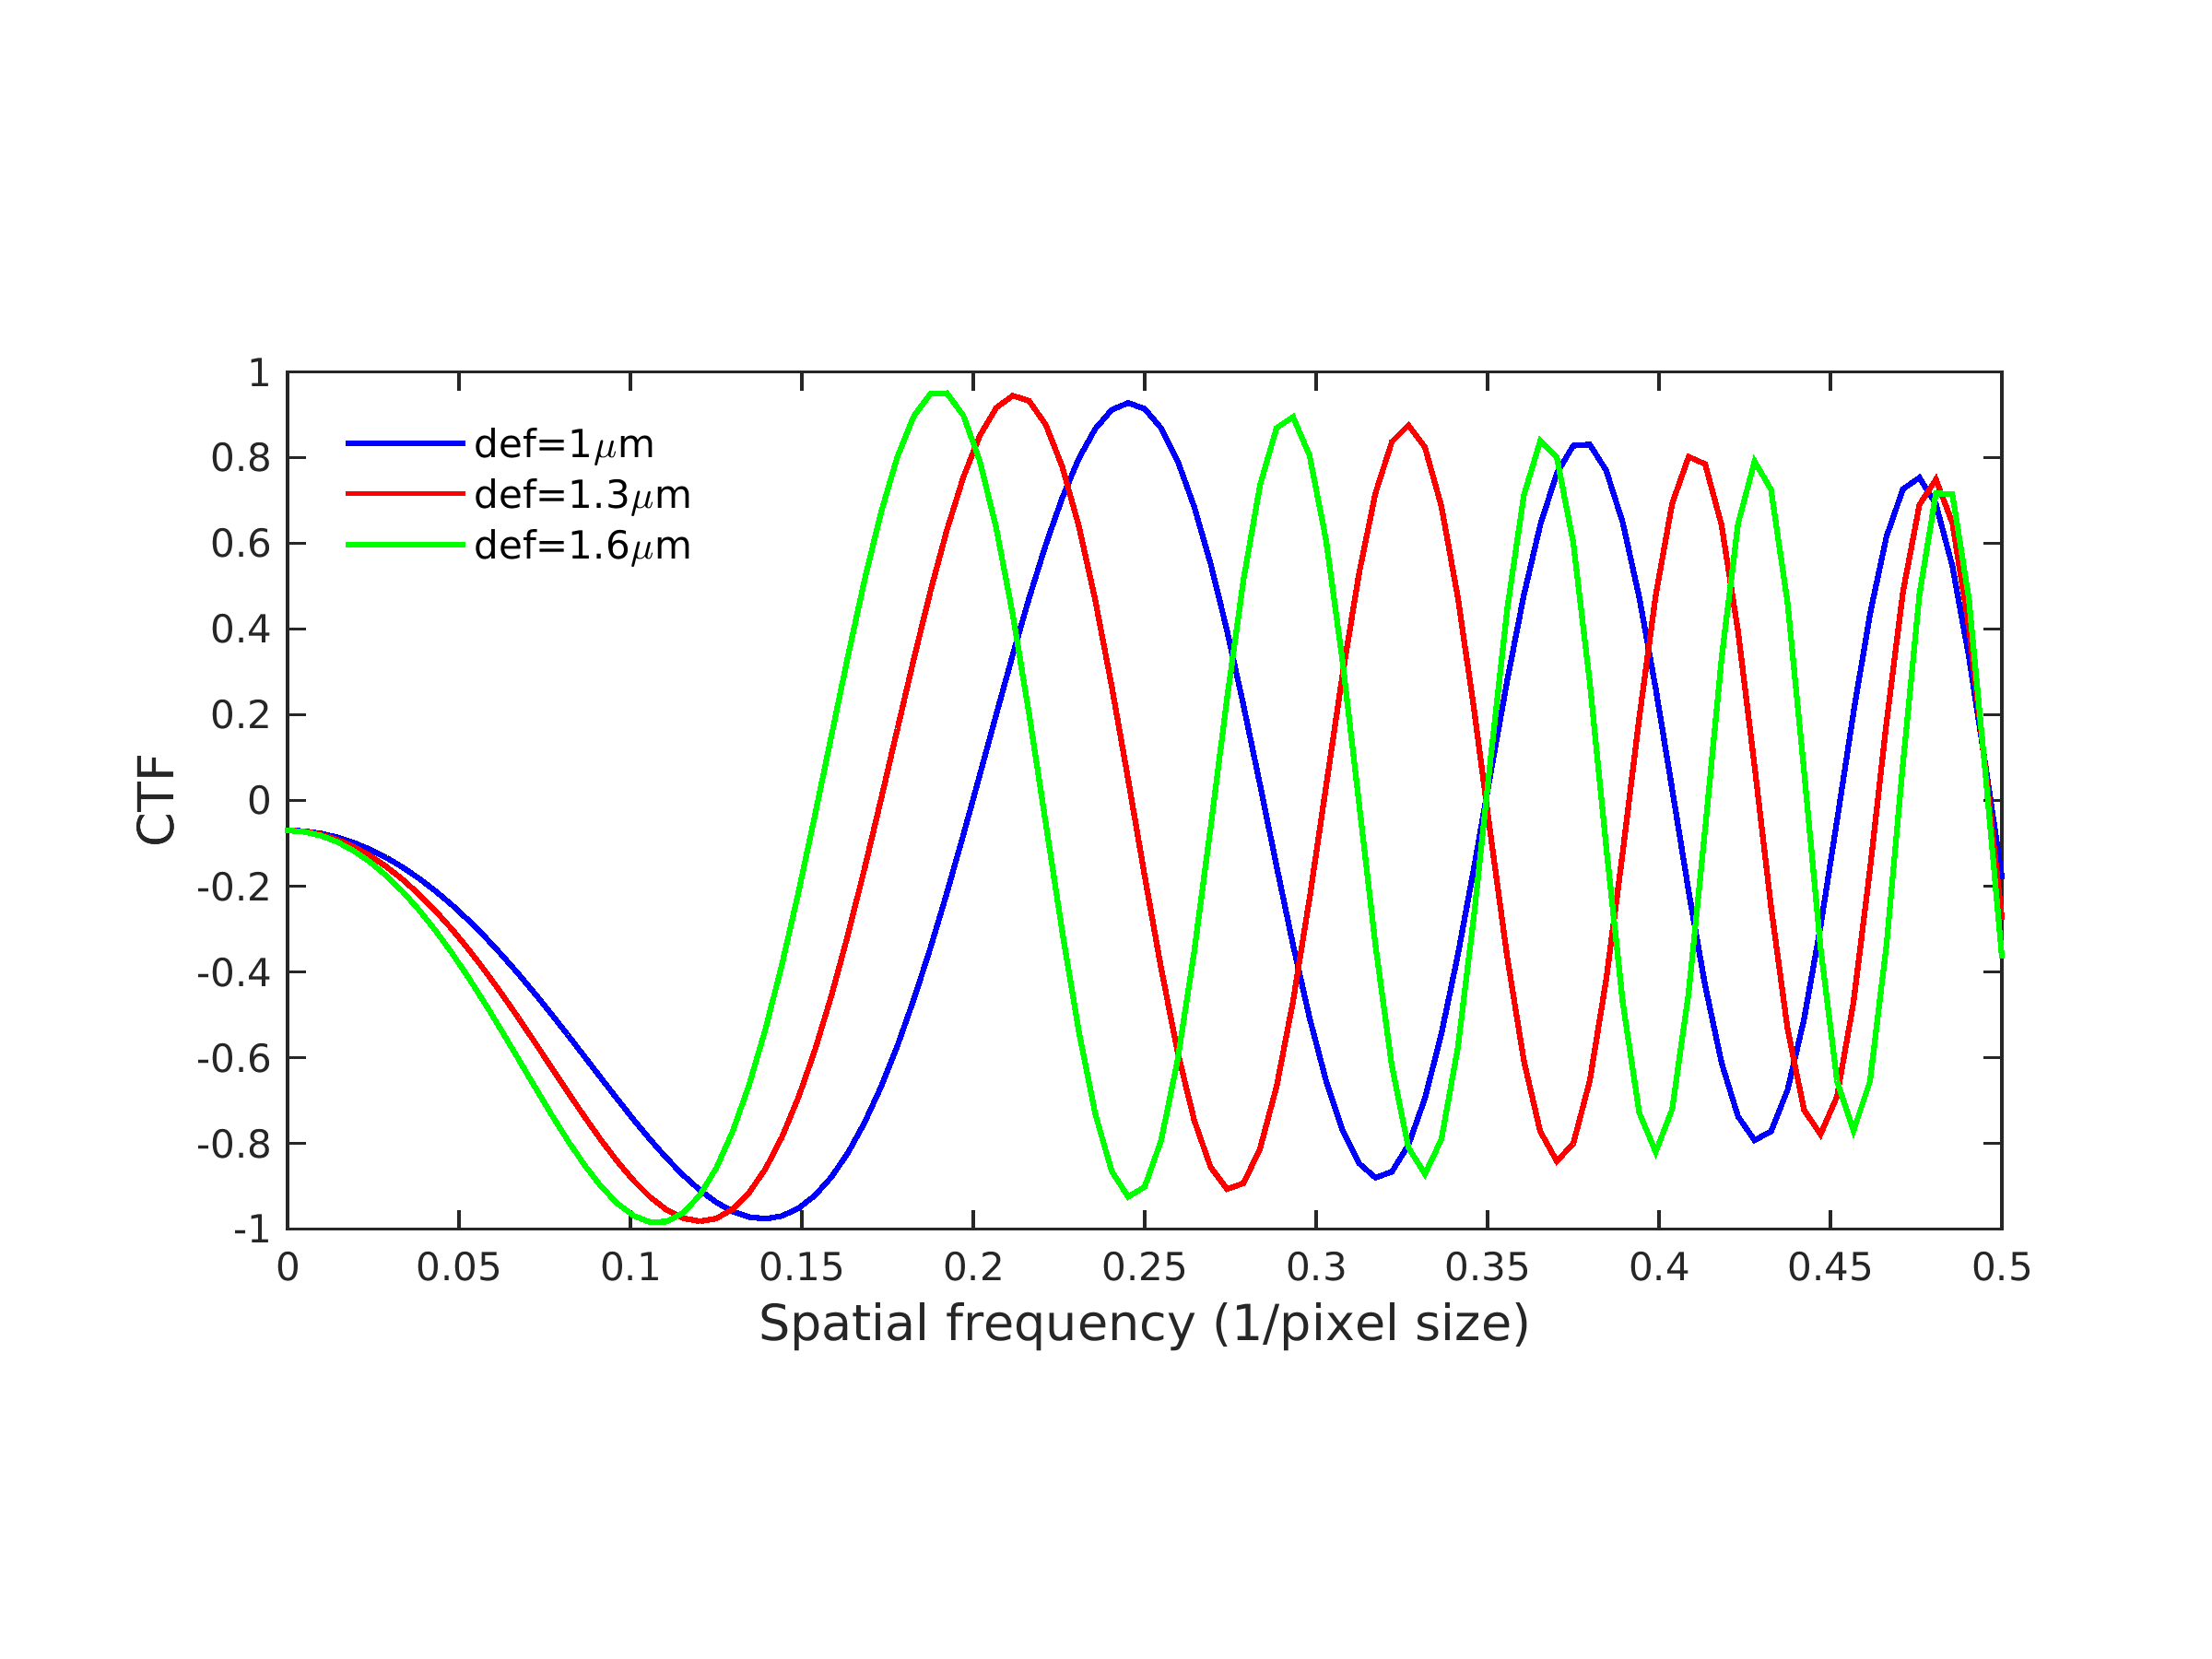
\includegraphics[scale=0.5]{ctfeg_fig.png}
\caption{CTF's for different values of the defocus.}\label{fig:ctf}
\end{center}

\end{figure}


\subsection{Class Averaging}
The procedure for class averaging, described in \cite{zhao}, consists of 3 main steps. First, Fourier Bessel Steerable PCA is used to denoise images and estimate the 2D covariance matrix of the images and their in-plane rotations. Phase flipping is used as a CTF correction scheme. Second, the bispectrum of the expansion coefficients in the steerable basis is computed. The bispectrum is a rotationally invariant representation of images, but is typically of very high dimensionality. It is projected on to a lower dimensional subspace using a fast, randomized PCA algorithm. One way to compare the distance between images after this step is to use the normalized cross correlation. However, this method suffers from outliers in the nearest neighbor detection at very low SNR's. So, the third step uses Vector Diffusion Maps to improve the initial classification by viewing angles.


\subsection{Covariance Wiener Filtering (CWF)}
CWF was proposed in \cite{cwf} as an algorithm to (i) estimate the CTF-corrected covariance matrix of the underlying clean 2D projection images and (ii) using the estimated covariance to solve the associated deconvolution problem in \ref{eq:imfour} to obtain denoised images, that are estimates of $X_i$ for each $i$ in 
\ref{eq:imfour}. The first step involves estimating the mean image of the dataset, $\mu$, as $\hat{\mu}$, followed by solving a least squares problem to estimate the covariance $\Sigma$ as $\hat{\Sigma}$. Under the assumption of additive white Gaussian noise, the estimate of the underlying clean image $X_i$ is given by
\begin{equation}
\hat{X_i}=(I-H_iA_i)\hat{\mu} + H_iY_i
\end{equation}
%
%\subsection{Fourier Bessel Steerable PCA}
%For both class averaging and CWF, the images are expressed in the Fourier Bessel basis. Since the basis elements are outer products of radial functions and angular Fourier modes, the covariance matrix is block diagonal in this choice of basis. Therefore each block of the covariance, corresponding to a particular angular frequency, can be computed separately, making the computation more efficient.
\section{Mahalonobis Distance}
Our goal is to define a metric to compare how close a any two cryo-EM images are, that is, given the CTF-affected, noisy observations for a pair of images
\begin{eqnarray} 
Y_i=H_i X_i + N_i, \quad \text{for} \quad i=1,2 .
%Y_2=H_2 X_2 + N_2 \nonumber,
\end{eqnarray}
Due to the numerous zero crossings of the CTF, CTF correction is a challenging problem. A popular albeit heuristic approach for CTF correction is 'phase flipping', which involves simply inverting the sign of the Fourier coefficients. This corrects for the phase inversion caused due to the CTF, but not for amplitude correction. In \cite{cwf}, the authors introduced a new approach for denoising and CTF correction in a single step, called CWF. When comparing distances between cryo-EM images, one must take into account that different images belong to different defocus groups, that is, they are affected by different CTF's. Since phase flipping is suboptimal as a method for CTF correction, computing nearest neighbors using the Euclidean distance between features constructed from phase flipped, denoised images can also suffer from incorrectly identified neighbors. The main motivation of this paper is to introduce a Mahalanobis distance for cryo-EM images, as a metric to compute the distance between images belonging to different defocus groups. Moreover, we propose to use this notion of distance to improve the existing class averaging pipeline in \cite{zhao1}.

We define a metric that gives a notion of distance between two underlying clean images $X_1$ and $X_2$. In our statistical model, the underlying clean images $X_1, X_2, \ldots X_n$ (where $n$ is the total number of images) are assumed to be independent, identically distributed (i.i.d.) samples drawn from a Gaussian distribution. Further, we assume that the noise in our model is additive white Gaussian noise.
\begin{eqnarray} 
X_1, X_2  \sim N( {\mu},\Sigma) \nonumber \\ 
N_1, N_2  \sim N(0,{\sigma}^2 I_n )
\end{eqnarray}

We denote the covariance of $Y_1$ and $Y_2$ by $K_1$ and $K_2$.
\begin{eqnarray}
% E(Y_1)=H_1 \mu \\ 
Cov(Y_i) = H_i \Sigma {H_i}^T + {\sigma}^2 I_n = K_i,\quad \text{for} \quad i=1,2 
%E(Y_2)=H_2 \mu \\
%Cov(Y_2) = H_2 \Sigma {H_2}^T + {\sigma}^2 I_n = K_2 
\end{eqnarray}
Using the Guassian property, we have the following probability density functions (pdf)
\begin{equation}
\small{
f_{X_i}(x_i) = P \exp\{-\frac{1}{2}{(x_i-\mu)}^T {\Sigma}^{-1}(x_i-\mu)\},\tiny{\quad\text{for}\quad i=1,2 }}
\end{equation}
%\begin{equation}
%\small{f_{X_2}(x_2) = P \exp\{-\frac{1}{2}{(x_2-\mu)}^T {\Sigma}^{-1}(x_2-\mu)\} }
%\end{equation}
\begin{equation}
\small{f_N(z_i) = Q \exp\{-\frac{1}{2}{(z_i)}^T \frac{1}{\sigma^2}(z_i)\}, z_i=y_i-H_1 x_i,\tiny{\quad\text{for}\quad i=1,2 }}
\end{equation}
%\begin{equation}
%\small{f_N(z_2) = Q \exp\{-\frac{1}{2}{(z_2)}^T \frac{1}{\sigma^2} (z_2)\}, z_2=y_2-H_2 x_2}
%\end{equation}
\begin{equation}
\small{f_{Y_i}(y_i) = R \exp\{-\frac{1}{2}{(y_i-H_i\mu)}^T {K_1}^{-1}(y_i-H_i\mu)\},\tiny{\quad\text{for}\quad i=1,2 } }
\end{equation}
%\begin{equation}
%\small{f_{Y_2}(y_2) = R \exp\{-\frac{1}{2}{(y_2-H_2\mu)}^T {K_2}^{-1}(y_2-H_2\mu)\}}
%\end{equation}
where $P=\frac{1}{({2\pi})^{\frac{n}{2}}{|\Sigma|}^{\frac{1}{2}}}$, $Q=\frac{1}{({2\pi})^{\frac{n}{2}}\sigma^n}$, and $R=\frac{1}{({2\pi})^{\frac{n}{2}} {|K_1|}^{\frac{1}{2}}}$.
\begin{equation}
 \left[\begin{array}{c} X_1 \\ Y_1 \end{array}\right] = 
\begin{bmatrix} I & 0 \\ H_1 & I \end{bmatrix} \times \left[ \begin{array}{c} X_1 \\ N_1 \end{array} \right]      
\end{equation}
\begin{equation}
 \sim N \left[\begin{bmatrix} \mu \\ H_1 \mu \end{bmatrix}, \begin{bmatrix} \Sigma & \Sigma H_1^T \\ H_1 \Sigma & H_1 \Sigma H_1^T + \sigma^2 I \end{bmatrix} \right]
\end{equation}
\noindent
Using conditional distributions
 \begin{equation}
  f_{X_1|Y_1}(x_1|y_1) \sim N(\alpha, L)
 \end{equation}
\begin{equation}
  f_{X_2|Y_2}(x_2|y_2) \sim N(\beta, M)
 \end{equation}
where 
\begin{equation}
\small{
\begin{array}{l}\alpha = \mu + \Sigma H_1^T (H_1 \Sigma H_1^T + \sigma^2 I)^{-1} (y_1 - H_1 \mu) \\ L = \Sigma - \Sigma H_1^T (H_1 \Sigma H_1^T + \sigma^2 I)^{-1} H_1 \Sigma \\ \beta = \mu + \Sigma H_2^T (H_2 \Sigma H_2^T + \sigma^2 I)^{-1} (y_2 - H_2 \mu) \\ M = \Sigma - \Sigma H_2^T (H_2 \Sigma H_2^T + \sigma^2 I)^{-1} H_2 \Sigma        \end{array}}   .
\end{equation}
So
\begin{equation}
P(x_1 - x_2|y_1, y_2) \sim N(\alpha-\beta, L+M)
\end{equation}
Let $x_1 - x_2 = x_3$, and $\alpha -\beta=\gamma$. Then
\begin{align}
&P(||x_3||_{\infty} < \epsilon|y_1,y_2)   \nonumber
										 =	 P(||x_3||_{\infty} < \epsilon|y_1,y_2)\\ \nonumber
										&=   \frac{1}{(2 \pi)^{\frac{n}{2}} |L+M|^ \frac{1}{2}} \times \\ 
										& \int_{-\epsilon }^{\epsilon}\exp \{ -\frac{1}{2}(x_3 - \gamma)^T(L+M)^{-1}(x_3 - \gamma\}dx_3 
\end{align}
For small $\epsilon$ this is
\begin{equation}
= \frac{(2 \epsilon)^n}{(2 \pi)^{\frac{n}{2}} |L + M|^{\frac{1}{2}}} \exp\{-\frac{1}{2}\gamma^T(L+M)^{-1}\gamma\} 
\label{eqn:metr}
\end{equation}
So we can define our metric after taking the logarithm on both sides of eqn.(\ref{eqn:metr}), dropping out the constant term, and substituting back $\gamma$
\begin{equation}
 -\frac{1}{2}\log(|L + M|) -\frac{1}{2}(\alpha - \beta)^T(L+M)^{-1}(\alpha -\beta)
\end{equation}


\section{Algorithm for Improved Class Averaging using Mahalanobis Distance}

We propose an improved class averaging algorithm that incorporates the Mahalanobis distance. The quantities $\alpha$, $\beta$, $L$, $M$ are computed for each image and defocus group respectively, using CWF \cite{cwf}. The estimated covariance using CWF is block diagonal in the Fourier Bessel basis. In practice, we use $\alpha$, $\beta$, $L$, $M$ projected onto the subspace spanned by the principal components (for angular frequency block). We obtain an initial list of $S$ nearest neighbors for each image using the Initial Classification algorithm in \cite{zhao1}. Then, for the list of nearest neighbors corresponding to each image, the Mahalanobis distance is computed and used to pick the closest $K$ nearest neighbors, where $K<S$. The details of the algorithm are listed in Algorithm \ref{alg:classav}. 

\begin{algorithm}
\caption{Improved Class Averaging }
\label{alg:classav}
\begin{algorithmic}[1]
\Procedure{Initial Classification \cite{zhao1}}{}
\State Image compression and denoising: compute Fourier Bessel steerable basis for images \cite{ffbspca}
\State Rotationally invariant features: compute the bispectrum from denoised coefficients in the steerable basis
\State Randomized PCA\cite{rokhlin} of high dimensional feature vectors from the bispectrum
\State Initial nearest neighbor classification and alignment using brute force or fast randomized approximate nearest neighbor search \cite{fastnn}
\State (Optional) Improve nearest neighbor classification using Vector Diffusion Maps (VDM) \cite{vdm}
\State Obtain a list of $S$ nearest neighbors for each image
\EndProcedure
\Procedure{Classification using Mahalonobis Distance}{}
\State Compute the quantities $\alpha, \beta, L, M$ using Covariance Wiener Filtering (CWF) \cite{cwf}
\State For each image and its $S$ aligned nearest neighbors, compute the Mahalanobis distance between the image and neighbors
\State Rank $S$ neighbors according to the Mahalanobis distance, and choose the top $K$ as nearest neighbors
\EndProcedure
\end{algorithmic}
\end{algorithm}


\section{Numerical experiments}

We test the improved class averaging algorithm on a synthetic dataset that consists of projection images generated from the volume of P. falciparum 80S ribosome bound to E-tRNA, available on the Electron Microscopy Data Bank (EMDB) as EMDB 6454.The algorithm was implemented in the UNIX environment, on a machine with total RAM of 1.5 TB, running at 2.3 GHz, and with 60 cores. 
For the results described here, we used $10000$ projection images of size $65 \times 65$ that were affected by the various CTF's and additive white Gaussian noise at various noise levels, in particular, we shoud here results for 4 values of the SNR. The images were divided into $20$ defocus groups. Initial classification was first used to select $S=50$ nearest neighbors for each image. After rotationally aligning the neighbors, the Mahalanobis distance was computed between each image and its $50$ aligned nearest neighbors. We then pick the closest $K=10$ neighbors for each image. For comparison, we compute $10$ nearest neighbors for each image using only Initial Classification (with or without using the optional VDM step). Table \ref{table:1} shows the number of pairs of nearest neighbor images detected with each method at various SNR's, that have correlation $>0.9$ between the original clean images, indicating that they are indeed neighbors. We note an improvement in the quality of nearest neighbors detected by the improved classification algorithm using the Mahalanobis distance. Figure \ref{fig:hist} shows the estimated probability density function of the angular distance between nearest neighbor images, using 1) Initial Classification only 2) Improved classification using the Mahalanobis distance. 

\begin{table}[]
\centering
\caption{Number of nearest neighbors with correlation $>0.9$, 
using 10000 images, $K=10$ and $S=50$.
}
\label{table:1}
\begin{tabular}{lllll}
      & \multicolumn{2}{l}{VDM} & \multicolumn{2}{l}{No VDM} \\ \cline{2-5} 
SNR   & New        & Old        & New          & Old         \\ \cline{2-5} 
%1/40 & 58361          & 56758          & 56831            & 49347       \\
1/60  & 34965          & 32113          & 34537            & 29219       \\
1/100 & 17262      & 14431      & 16057        & 13706        \\ \cline{2-5} 
\end{tabular}
\end{table}


\begin{figure}[!htbp]
\begin{center}
\begin{tabular}{cc}
\includegraphics[width=.49\columnwidth]{fighist_snr1by20.png} & \includegraphics[width=.49\columnwidth]{fighist_snr1by40.png} \\
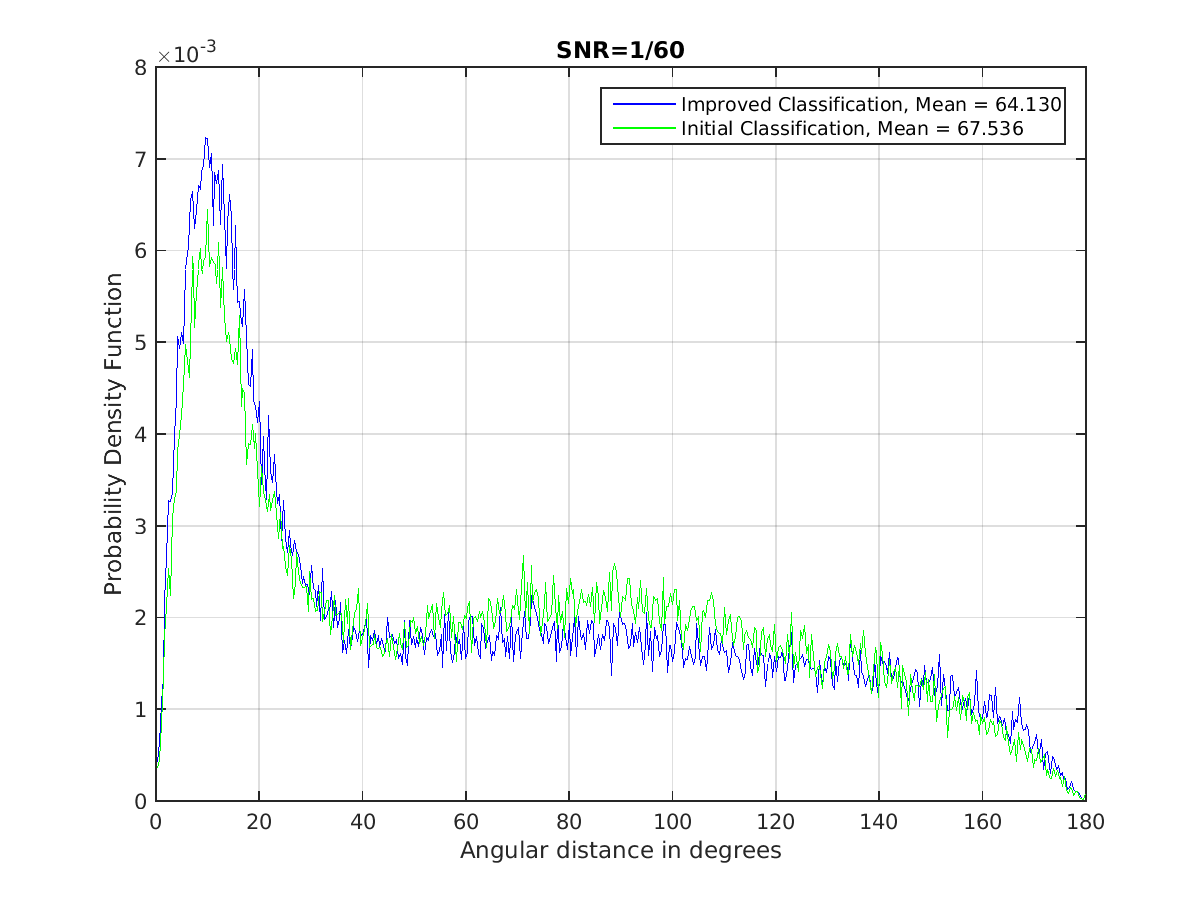
\includegraphics[width=.49\columnwidth]{fighist_snr1by60.png} & 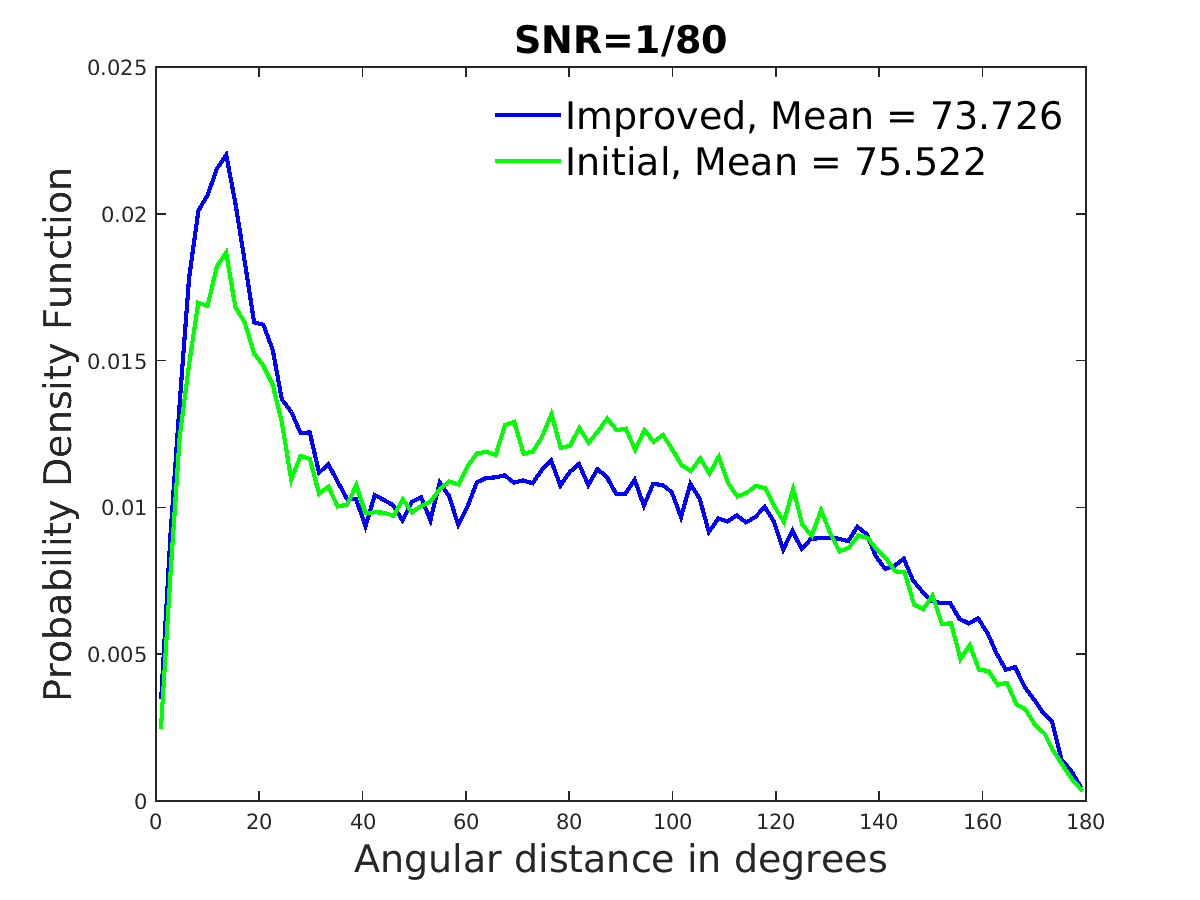
\includegraphics[width=.49\columnwidth]{fighist_snr1by80.png}
\end{tabular}
\end{center}
\caption{The estimated probability density function of the angular distance (in degrees) between images classified into the same class by 1) Initial Classification and 2) Improved Classification using the Mahalanobis distance at different SNR's.}
\label{fig:hist}
\end{figure}

\section{Future Work}
The Mahalonobis distance proposed here can be used as a metric for any manifold learning procedure \cite{intgeom, nlica} such as diffusion maps \cite{vdm, difmap}, with or without missing data.

\section{Conclusion}



% References should be produced using the bibtex program from suitable
% BiBTeX files (here: strings, refs, manuals). The IEEEbib.bst bibliography
% style file from IEEE produces unsorted bibliography list.
% -------------------------------------------------------------------------
\bibliographystyle{IEEEbib}
\bibliography{cwf_isbi_ref}


\end{document}

% \begin{figure}
% \centering
% \begin{subfigure}{.25\textwidth}
%   \centering
%   \includegraphics[width=.7\linewidth]{noise07alpha.png}
%   \caption{OR: $\alpha_4$ known}\label{fig:noisealpha}
%   \label{fig:sub1}
% \end{subfigure}%
% \begin{subfigure}{.25\textwidth}
%   \centering
%   \includegraphics[width=.7\linewidth]{noise07beta.png}
%   \caption{OR: $\beta_4$ known}\label{fig:noisebeta}
%   \label{fig:sub2}
% \end{subfigure}
% \caption{Reconstruction from noisy images. SNR=0.7}
% \label{fig:noisy}
% \end{figure}
% \begin{figure}
% \centering
% \begin{subfigure}{.25\textwidth}
%   \centering
%   \includegraphics[width=.7\linewidth]{noise035alpha.png}
%   \caption{OR: $\alpha_4$ known}\label{fig:noisealpha035}
%   \label{fig:sub1}
% \end{subfigure}%
% \begin{subfigure}{.25\textwidth}
%   \centering
%   \includegraphics[width=.7\linewidth]{noise035beta.png}
%   \caption{OR: $\beta_4$ known}\label{fig:noisebeta035}
%   \label{fig:sub2}
% \end{subfigure}
% \caption{Reconstruction from noisy images. SNR=0.35}
% \label{fig:noisy035}
% \end{figure}
% \begin{figure}
% \centering
% \begin{minipage}{.2\textwidth}
%   \centering
%   \includegraphics[width=.5\linewidth]{noise07alpha.png}
%   \caption{OR: $\alpha_4$ known}\label{fig:noisealpha}
%   \label{fig:test1}
% \end{minipage}%
% \begin{minipage}{.2\textwidth}
%   \centering
%   \includegraphics[width=.5\linewidth]{noise07beta.png}
%   \caption{OR: $\beta_4$ known}\label{fig:noisebeta}
%   \label{fig:test2}
% \end{minipage}
% \end{figure}


% \includegraphics[width=.49\columnwidth]{cat_alpha.png} \includegraphics[width=.49\columnwidth]{cat_beta}
% \begin{figure}
% \centering
% \begin{subfigure}{.25\textwidth}
%   \centering
%   \includegraphics[width=.49\columnwidth]{cat_alpha.png} \includegraphics[width=.49\columnwidth]{cat_beta}
%   \caption{Reconstruction from clean images. Top left: OE with $\alpha_4$ known. Top right: OE with $\beta_4$ known}
%   \label{fig:sub1}
% \end{subfigure}%
% \begin{subfigure}{.25\textwidth}
%   \centering
%   \includegraphics[width=.7\linewidth]{cat_beta.png}
%   \caption{OE: $\beta_4$ known}\label{fig:catbeta}
%   \label{fig:sub2}
% \end{subfigure}
% \caption{Reconstruction from clean images using OE}
% \label{fig:cleanOE}
% \end{figure}
% \begin{figure}
% \centering
% \begin{subfigure}{.25\textwidth}
%   \centering
%   \includegraphics[width=.7\linewidth]{sdpalpha.png}
%   \caption{OR: $\alpha_4$ known}\label{fig:sdpalpha}
%   \label{fig:sub1}
% \end{subfigure}%
% \begin{subfigure}{.25\textwidth}
%   \centering
%   \includegraphics[width=.7\linewidth]{sdpbeta.png}
%   \caption{OR: $\beta_4$ known}\label{fig:sdpbeta}
%   \label{fig:sub2}
% \end{subfigure}
% \caption{Reconstruction from clean images using OR}
% \label{fig:cleanOR}
% \end{figure}


% \begin{figure}
% \centering
% \begin{subfigure}{.25\textwidth}
%   \centering
%   \includegraphics[width=.7\linewidth]{truth.png}
%   \caption{}
%   \label{fig:kvtrue}
% \end{subfigure}%
% \begin{subfigure}{.25\textwidth}
%   \centering
%   \includegraphics[width=.7\linewidth]{kv12.PNG}
%   \caption{}
%   \label{fig:kvscheme}
% \end{subfigure}
% \caption{Kv1.2 potassium channel}
% \label{fig:truth}
% \end{figure}
% \begin{figure}
% \centering
% \begin{minipage}{.2\textwidth}
%   \centering
%   \includegraphics[width=.5\linewidth]{cat_alpha.png}
%   \caption{OE: $\alpha_4$ known}\label{fig:catalpha}
%   \label{fig:test1}
% \end{minipage}%
% \begin{minipage}{.2\textwidth}
%   \centering
%   \includegraphics[width=.5\linewidth]{cat_beta.png}
%   \caption{OE: $\beta_4$ known}\label{fig:catbeta}
%   \label{fig:test2}
% \end{minipage}
% \end{figure}

%  One approach to solve
% (\ref{noncon}) is to use an alternating least squares (ALS) procedure, which is
% an iterative procedure that alternates
% between updating $O_l^{(1)}$ and $O_l^{(2)}$.
% \begin{equation*}\label{noncon}
% O_l^{(1)} \leftarrow \argmin_{O_l^{(1)} \in O(2l+1)}
% ||F_l^{(2)}-F_l^{(1)}-G_l^{(2)}O_l^{(2)}-G_l^{(1)}O_l^{(1)} ||_F^2
% \end{equation*}
% \begin{equation}\label{noncon}
% O_l^{(2)} \leftarrow \argmin_{O_l^{(1)} \in O(2l+1)}
% ||F_l^{(2)}-F_l^{(1)}-G_l^{(2)}O_l^{(2)}-G_l^{(1)}O_l^{(1)} ||_F^2
% \end{equation}
% These update rules have a closed form solution using singular value
% decomposition. Each iteration reduces the value of
% the cost function in (\ref{noncon}), so the iterates converge to a local but non
% necessarily global minimum. Numerical
% simulations show that ALS does not converge to a global minimum unless we start
% with a good initialization. 
